\chapter{Architektura zaproponowanego rozwiązania}
\label{cha:arch}

W niniejszej pracy została zaproponowana hybrydowa struktura aplikacji realizującej zadania wyliczania i aplikowania sterowania czasooptymalnego, jak i minimalnego w sensie liniowo-kwadratowego wskaźnika jakości.
Taka jej architektura jest odbiciem faktycznej tendencji w automatyce ostatnich lat: aby skomplikowane zadania obliczeniowe zadawać nie tym elementom, które realizują bezpośrednie sterowanie, ale zlecać je innym urządzeniom o architekturze sprzętu odpowiedniejszej do radzenia sobie z takimi problemami.

Dokładnie takie podejście zostało również zaprezentowane w niniejszej pracy. Hybrydowa (z łaciny: \emph{hybrida}: mieszaniec, krzyżówka) struktura polega na zastosowaniu dwóch poziomów: obliczeniowego i realizującego sterowanie bezpośrednie. Zostały one szerzej opisane w tym rozdziale.

\section{Podział zadań między elementami oprogramowania}
\label{sec:podzial-zadan}

W związku z zaproponowaną w niniejszej pracy architekturą oprogramowania, opierającą się na dwóch poziomach, kluczowym aspektem tego opracowania jest odpowiedni podział zadań między tymi poziomami.

Pierwszy z nich to część ,,wyższego poziomu'' - została tak określona ze względu na to, iż nie ma bezpośredniego wpływu na kontrolowany fizyczny obiekt, a zajmuje się tylko modelem matematycznym. Jej zadania są przedstawione na poniższej liście.

\begin{enumerate}
    \item Symulacja modelu nieliniowego w pętli otwartej, aby zainicjować algorytm optymalizacji dynamicznej.
    \item Wyznaczanie sterowania czasooptymalnego dla zadanych wartości początkowych i końcowych.
    \item Symulacja modelu nieliniowego w pętli zamkniętej, aby zweryfikować wyliczone sterowanie czasooptymalne.
    \item Linearyzacja modelu w punkcie pracy.
    \item Wyznaczanie sterowania optymalnego w sensie liniowo-kwadratowego wskaźnika jakości (dla modelu linearyzowanego w punkcie pracy).
\end{enumerate}

Dodatkowo przyjęto następujące założenia w związku z tymi zadaniami (podzielone ze względu na to, którego zagadnienia optymalizacji dotyczą):

\begin{enumerate}
    \item Założenia związane ze sterowaniem czasooptymalnym:
    \begin{enumerate}
        \item Sterowanie czasooptymalne jest postaci ,,bang-bang'' (wyjaśnienie w sekcji \ref{sub:toc-nonlnr}).
        \item W związku z tym wystarczy wyznaczyć czasy przełączeń między konkretnymi sterowaniami maksymalnym i minimalnym oraz to, które z nich ma być aplikowane jako pierwsze.
    \end{enumerate}
    \item Założenia związane ze sterowaniem liniowo-kwadratowym:
    \begin{enumerate}
        \item Punkt pracy (w którym jest dokonywana linearyzacja) jest stanem docelowym zagadnienia czasooptymalnego, jeśli ten jest punktem równowagi systemu (definicja dana w podrozdziale \ref{sec:model}).
        \item Jeśli stan docelowy zagadnienia czasooptymalnego nie jest stanem ustalonym rozważanego układu, stosuje się przybliżenie go do pewnego punktu równowagi i tam dokonuje się linearyzacji modelu matematycznego.
        \item Sterowanie liniowo-kwadratowe jest wyliczane jako odchyłka od sterowania ustalonego dla punktu równowagi.
    \end{enumerate}
\end{enumerate}

Na podstawie powyższych zadań oraz założeń sformułowano poniższą listę parametrów, które musi przyjmować część optymalizacyjna od użytkownika:

\begin{itemize}
    \item parametry statyczne modelu matematycznego:
    \begin{itemize}
        \item fizyczne rozmiary zbiorników (parametry $a$, $b$, $c$, $R$, $w$ i $h_{max}$),
        \item opory wypływu ze zbiorników (parametry $C_{1}$, $C_{2}$ oraz $C_{3}$),
        \item współczynniki wypływu ze zbiorników(parametry $\alpha_{1}$, $\alpha_{2}$ i $\alpha_{3}$);
    \end{itemize}
    \item wielkości związane z ograniczeniami w zagadnieniu czasooptymalnym:
    \begin{itemize}
        \item maksymalne sterowanie ($u_{max}$),
        \item wartości początkowe poziomów wody w zbiornikach (parametry $h_{10}$, $h_{20}$ oraz $h_{30}$),
        \item wartości końcowe poziomów wody w zbiornikach (parametry $h_{1f}$, $h_{2f}$ i $h_{3f}$);
    \end{itemize}
    \item wagi w zagadnieniu liniowo-kwadratowym:
    \begin{itemize}
        \item wartość wagi sterowania $R \in \mathbb{R}$,
        \item wartości wag stanów dane jako macierz $Q \in \mathbb{R}^{3}$.
    \end{itemize}
\end{itemize}

Drugi poziom zaproponowanego w niniejszej pracy rozwiązania to część ,,niższego poziomu'' - jej nazwa jest związana z tym, że bezpośrednio wpływa na sterowany układ. Nie zawiera tak skomplikowanych narzędzi obliczeniowych, ale za to powinna cechować się dużą niezawodnością. Jej zadania są przedstawione na poniższej liście.

\begin{enumerate}
    \item Aplikacja sterowania czasooptymalnego przez czas, który jest wyliczony przez część ,,wyższego poziomu'' oraz w odpowiedniej postaci (,,bang-bang'').
    \item Po upływie tego czasu aplikacja sterowania optymalnego w sensie liniowo-kwadratowego wskaźnika jakości aż do czasu otrzymania kolejnego sterowania czasooptymalnego.
    \item Symulacja układu modelu matematycznego w celach testowych i weryfikacyjnych.
\end{enumerate}

W związku z tym, że jest to element realizujący bezpośrednie sterowanie, użytkownik nie powinien mieć wpływu na jego funkcjonowanie. Cały interfejs między nim a programem sterującym powinien dotyczyć tylko i wyłącznie części ,,wyższego poziomu''.


\section{Komunikacja między elementami oprogramowania}
\label{sec:komunikacja}

Hybrydowa struktura aplikacji wymusza dokładne zdefiniowanie schematów komunikacyjnych między oboma jej poziomami.
Poniżej znajduje się podsumowanie wartości wysyłanych przez oba poziomy.

\begin{enumerate} 
    \item Część obliczeniowa wysyła:
    \begin{enumerate}
        \item wartości końcowe poziomów w zbiornikach (będące stanem docelowym w zadaniu czasooptymalnym oraz punktem linearyzacji modelu służącym do wyliczenia nastaw regulatora liniowo-kwadratowego),
        \item dla regulatora czasooptymalnego:
        \begin{enumerate}
            \item czasy przełączeń (założono postać sterowania typu ,,bang-bang''),
            \item wartość początkową sterowania czasooptymalnego,
            \item wartość ,,drugorzędną'' tego sterowania (założono, że część ,,niższa'' nie musi znać ograniczeń nałożonych na sterowanie),
            \item czas aplikacji sterowania czasooptymalnego (będący wartością wskaźnika jakości w tym zadaniu);
        \end{enumerate}
        \item dla regulatora liniowo-kwadratowego:
        \begin{enumerate}
            \item wektor K współczynników regulatora,
            \item sterowanie ustalone, od którego są liczone odchyłki.
        \end{enumerate}
    \end{enumerate}
    \item Część sterowania bezpośredniego wysyła:
    \begin{itemize}
        \item aktualne poziomy wody w zbiornikach,
        \item aktualną wartość sterowania.
    \end{itemize}
\end{enumerate}

Wyszczególniono 3 możliwe akcje zachodzące w systemie, poniżej znajduje się ich lista. Zilustrowano je odpowiednimi (aczkolwiek uproszczonymi do poziomu ogólnej specyfikacji) diagramami sekwencji według konwencji UML. Wyszczególniono na nich użytkownika, część obliczeniową i sterującą oraz oprogramowanie optymalizacyjne, aby zaznaczyć, że jest ono de facto osobnym elementem, zewnętrznym i niestanowiącym części aplikacji będącej przedmiotem niniejszej pracy.

\begin{enumerate}
    \item Akcja obliczania sterowania czasooptymalnego (przedstawiona na rys. \ref{fig:comm-toc}).
    \item Akcja obliczania sterowania liniowo-kwadratowego (pokazana na rys. \ref{fig:comm-lqr}).
    \item Akcja wysłania obliczonych sterowań między poziomami aplikacji (zaprezentowana na rys. \ref{fig:comm-send} zawierającym pozostałe akcje w uproszczonej formie).
\end{enumerate}

\begin{figure}[hpt]
    \centering
    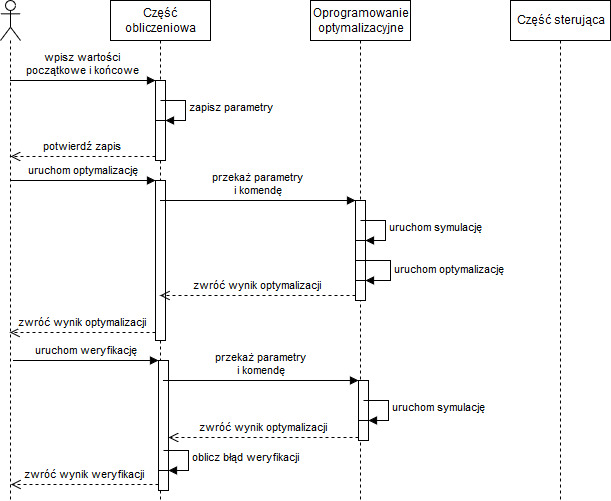
\includegraphics[width=\textwidth]{Grafika/communication-toc}
    \caption{Diagram sekwencji ilustrujący akcję obliczenia sterowania czasooptymalnego. Źródło: własne.}\label{fig:comm-toc}
\end{figure}

\begin{figure}[hpt]
    \centering
    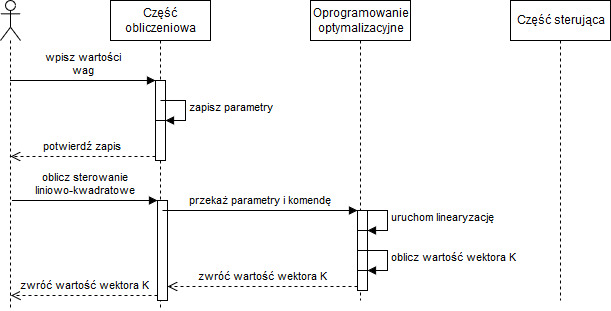
\includegraphics[width=\textwidth]{Grafika/communication-lqr}
    \caption{Diagram sekwencji ilustrujący akcję obliczenia sterowania liniowo-kwadratowego. Źródło: własne.}\label{fig:comm-lqr}
\end{figure}

\begin{figure}[hpt]
    \centering
    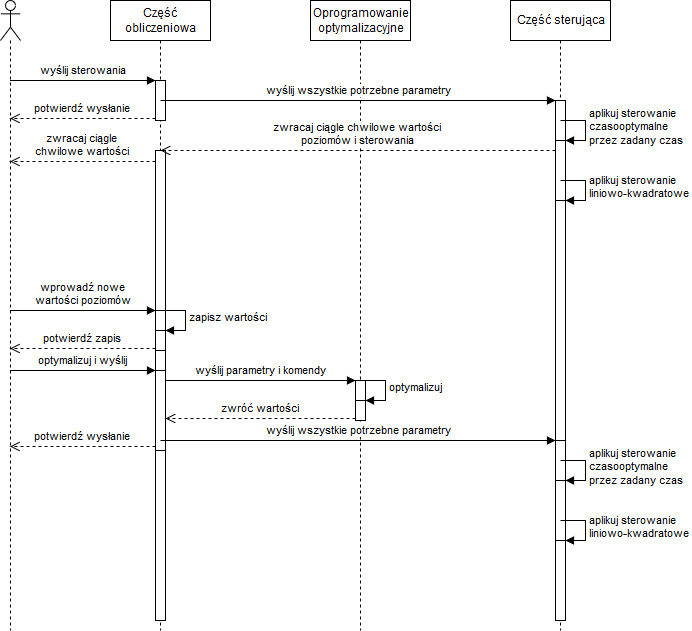
\includegraphics[width=\textwidth]{Grafika/communication-between-levels}
    \caption{Diagram sekwencji ilustrujący akcję wysyłania sterowań. Źródło: własne.}\label{fig:comm-send}
\end{figure}
